\section{ОПИСАНИЕ МОДЕЛИ ОБЪЕКТА АВТОМАТИЗАЦИИ}
\subsection{Организационная модель}

\textbf{Организационная структура} - совокупность подразделений организации и их взаимосвязей,
в рамках которой между подразделениями распределяются функциональные задачи,
определяются полномочия и ответственность руководителей и должностных лиц.

Структура предприятия устанавливается исходя из объема и содержания задач,
решаемых предприятием, направленности и интенсивности сложившихся на предприятии
информационных и документационных потоков и с учетом его организационных и материальных возможностей.

Оргструктура представляется через органограмму и такие документы, как штатное расписание,
устав организации и пр.

\textbf{Органограмма} - графическое представление структуры организации.

Основные элементы организационной диаграммы (ARIS Express 2.4i \cite{ArisExpress} Organizational chart)
представлены на рисунке~\ref{fig:ArisOrganizationalChartElements}.

\begin{figure}[!h]
    \centering
    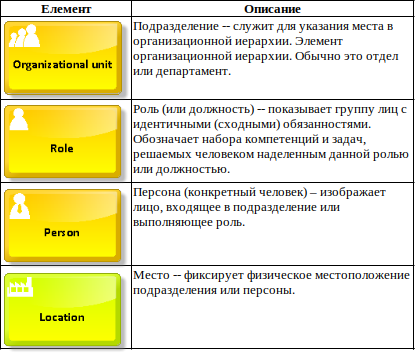
\includegraphics[width=12cm]
    {assets/ARIS/OrganizationalChart/Elements/ArisOrganizationalChartElements.png}
    \caption{Основные элементы организационной диаграммы}
    \label{fig:ArisOrganizationalChartElements}
\end{figure}

\newpage

Организационная модель ОА <<Косметический салон>> представлена органограммой
(см. рисунок~\ref{fig:ArisOrganizationalChart_all})
с использованием методологии ARIS нотации~ <<Orga\-nizational chart>>
(в ARIS Express 2.4i \cite{ArisExpress}),
а также таблицей <<Каталог организационных единиц>>
(см.~рисунок~\ref{fig:OrganizationalChartCatalog_all}).

\begin{figure}[!h]
    \centering

    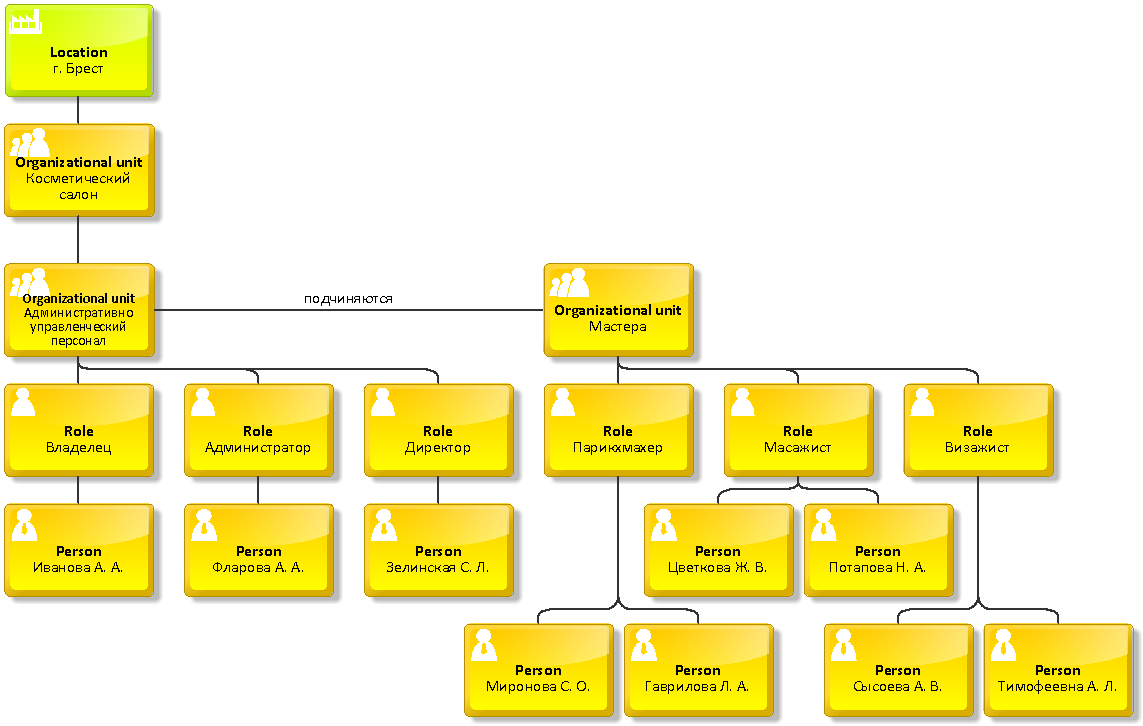
\includegraphics[width=16cm]
    {assets/ARIS/OrganizationalChart/all/ArisOrganizationalChart.png}

    \caption{Органограмма ОА <<Косметический салон>>}

    \label{fig:ArisOrganizationalChart_all}
\end{figure}

\begin{figure}[!h]
    \centering

    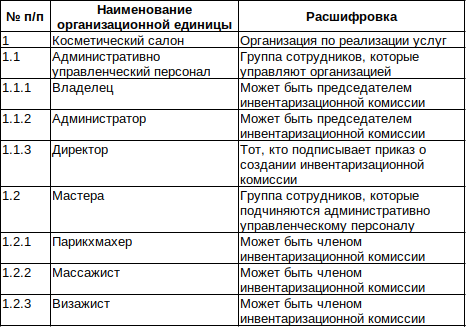
\includegraphics[width=11cm]
    {assets/ARIS/OrganizationalChart/all/OrganizationalChartCatalog.png}

    \caption{Каталог организационных единиц}

    \label{fig:OrganizationalChartCatalog_all}
\end{figure}

Организационная модель инвентаризационная комиссия представлена органограммой
(см.~рисунок~\ref{fig:ArisOrganizationalChart_comission})
с использованием методологии ARIS нотации <<Orga\-nizational chart>>
(в ARIS Express 2.4i \cite{ArisExpress}),
а также таблицей <<Каталог организационных единиц инвентаризационной комиссии>>
(см.~рисунок~\ref{fig:OrganizationalChartCatalog_comission}).

\begin{figure}[!h]
    \centering

    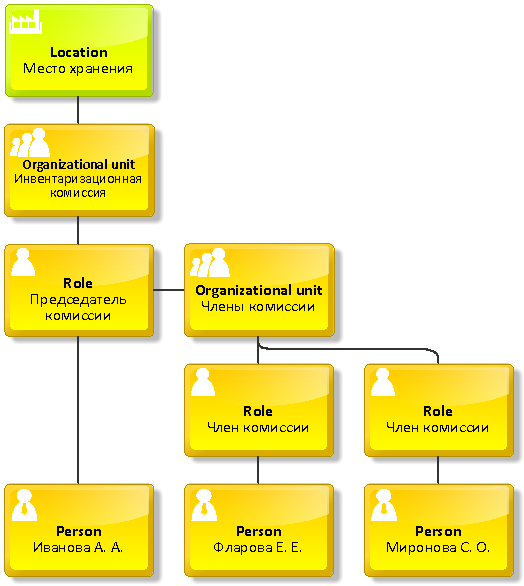
\includegraphics[width=12cm]
    {assets/ARIS/OrganizationalChart/comission/ArisOrganizationalChart.png}

    \caption{Органограмма инвентаризационной комиссии}

    \label{fig:ArisOrganizationalChart_comission}
\end{figure}

\begin{figure}[!h]
    \centering

    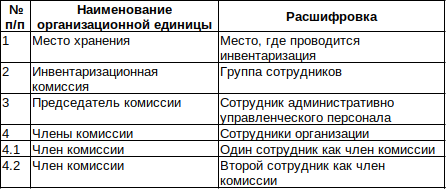
\includegraphics[width=11cm]
    {assets/ARIS/OrganizationalChart/comission/OrganizationalChartCatalog.png}

    \caption{Каталог организационных единиц}

    \label{fig:OrganizationalChartCatalog_comission}
\end{figure}

% = = = = = = = = = = = = = = = = = = = = = = = = = = = = = = = =

\newpage
\subsection{Функциональная модель}

\textbf{Функциональная модель объекта автоматизации} - описание его на языке выполняемых функций и их отношений.

\textbf{Функциональная структура} - структура, элементами которой являются функции,
реализуемые подразделениями предприятия, а отношениями являются связи,
обеспечивающие передачу между элементами предметов труда.

\textbf{Функция} - это предметно-ориентированное задание или действие,
в результате которой выполняется одна или несколько целей, стоящих перед компанией.
Функции предприятия распределяются по компонентам оргструктуры и представляют собой иерархическое дерево,
строящееся от общего к частному.
На самом верхнем уровне описываются самые сложные функции,
которые потом детализируются через свои функциональные составляющие.

Функциональная структура в методология ARIS представляется через нотацию VAD (Value Added Chain Diagram) или Process Landscape.
Данная нотация позволяет представлять функциональную структуру предприятия через иерархию и через последовательность (цепочку) процессов.
Основной символ карты процессов (ARIS Express 2.4i \cite{ArisExpress} Process landscape)
изображен на рисунке~\ref{fig:ProcessLandscapeElement}.

\begin{figure}[!h]
    \centering

    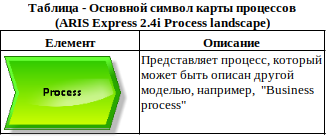
\includegraphics[width=12cm]
    {assets/ARIS/ProcessLandscape/Element/ProcessLandscapeElement.png}

    \caption{Основной символ карты процессов}

    \label{fig:ProcessLandscapeElement}
\end{figure}

Функциональная модель объекта автоматизации <<Косметический салон>> подсистемы <<Инвентаризация>>
соответствует организационной структуре и представлена
с использованием методологии ARIS нотации <<Process Landscape>>
(см.~рисунок~\ref{fig:ArisProcessLandscape}),
а также таблицей <<Каталог функций>>
(см.~рисунок~\ref{fig:ProcessLandscapeCatalog}).

\begin{figure}[!hp]
    \centering

    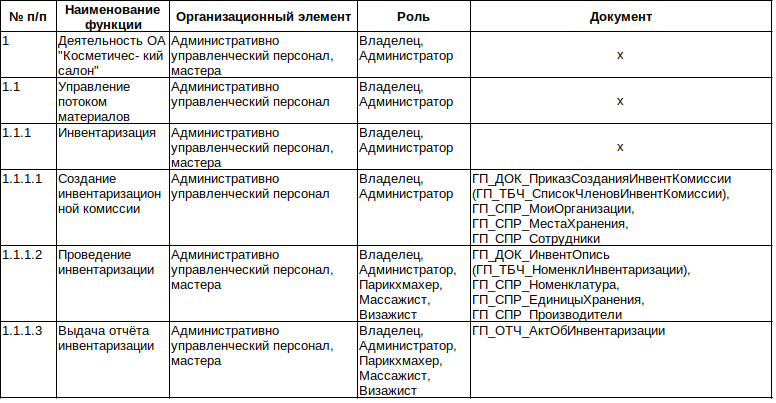
\includegraphics[height=8.5cm]
    {assets/ARIS/ProcessLandscape/ProcessLandscapeCatalog.png}

    \caption{Каталог функций}

    \label{fig:ProcessLandscapeCatalog}
\end{figure}

\begin{figure}[!hp]
    \centering

    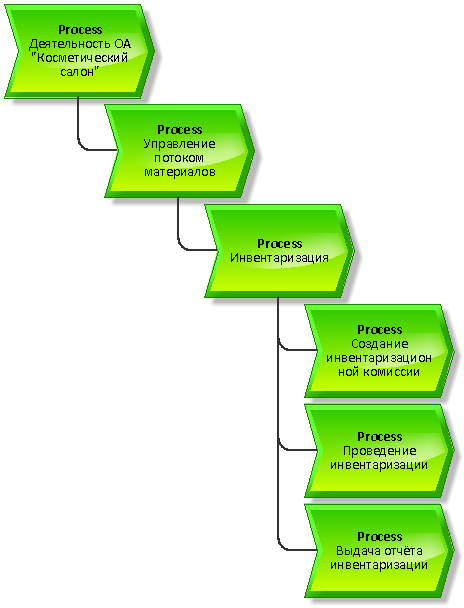
\includegraphics[height=14cm]
    {assets/ARIS/ProcessLandscape/ArisProcessLandscape.png}

    \caption{Функциональное дерево ОА <<Косметический салон>>}

    \label{fig:ArisProcessLandscape}
\end{figure}

% = = = = = = = = = = = = = = = = = = = = = = = = = = = = = = = =

\newpage
\subsection{Информационная модель}

\textbf{Информационная структура объекта автоматизации} - это совокупность документов, архивов,
правил и норм ведения документооборота, используемые на объекте автоматизации.
В информационной системе объекта автоматизации входят так же средства автоматизации
(автоматизированные и информационные системы, базы данных, электронные архивы),
используемые объектом.
Все элементы ИC ОА относятся либо к внемашинному (бумажному) либо внутримашинному (цифровому) обеспечению. 

\textbf{Информационная модель} - модель объекта, представленная в виде информации,
описывающей существенные для данного рассмотрения параметры и переменные величины объекта,
связи между ними, входы и выходы объекта и позволяющая путём подачи на модель информации об изменениях
входных величин моделировать возможные состояния объекта.

Информационная модель ОА <<Инвентаризация>> для ИС <<Косметический салон>> включает в себя следующие документы:

\begin{itemize}
    \item список справочных документов (см.~таблицу~\ref{fig:GP_CTL_catalog});
    \item список оперативных документов (см.~таблицу~\ref{fig:GP_DOC_catalog});
    \item список отчётных документов (см.~таблицу~\ref{fig:GP_REP_catalog}).
\end{itemize}

\begin{figure}[!h]
    \centering

    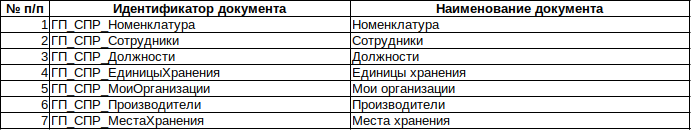
\includegraphics[width=15cm]
    {assets/ARIS/GeneralDiagram/ГП_СПР_.png}

    \caption{Каталог справочных документов}

    \label{fig:GP_CTL_catalog}
\end{figure}

\begin{figure}[!h]
    \centering

    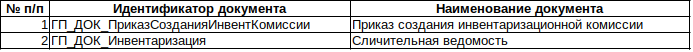
\includegraphics[width=15cm]
    {assets/ARIS/GeneralDiagram/ГП_ДОК_.png}

    \caption{Каталог оперативных документов}

    \label{fig:GP_DOC_catalog}
\end{figure}

\begin{figure}[!h]
    \centering

    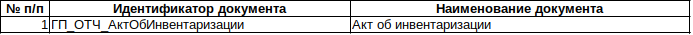
\includegraphics[width=15cm]
    {assets/ARIS/GeneralDiagram/ГП_ОТЧ_.png}

    \caption{Каталог отчетов}

    \label{fig:GP_REP_catalog}
\end{figure}

Основные элементы информационной модели методологии ARIS нотации <<General Diagram>>
представлены на рисунке~\ref{fig:GeneralDiagramElements}

\begin{figure}[!h]
    \centering

    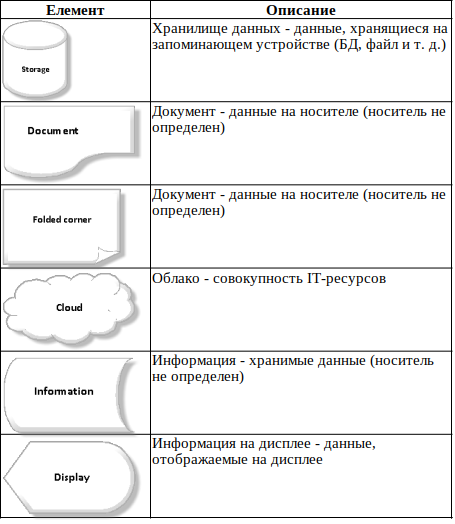
\includegraphics[width=13cm]
    {assets/ARIS/GeneralDiagram/Elements/GeneralDiagramElements.png}

    \caption{Основные элементы нотации General Diagram}

    \label{fig:GeneralDiagramElements}
\end{figure}

% = = = = = = = = = = = = = = = = = = = = = = = = = = = = = = = =

\subsubsection*{Оперативный документ <<Приказ о создании инвентаризационной комиссии>>}

Оперативный документ <<Приказ о создании инвентаризационной комиссии>>
- документ, который формируется перед инвентаризацией товара.
Документ представлен в виде
макета (см.~рисунок~\ref{fig:GP_DOC_Prikaz_layout}),
словаря данных (см.~рисунок~\ref{fig:GP_DOC_Prikaz_data}),
и схемы связей (см.~рисунок~\ref{fig:GP_DOC_Prikaz_relations}) представленной методологией ARIS нотацией <<General Diagram>>.

\begin{figure}[!hp]
    \centering

    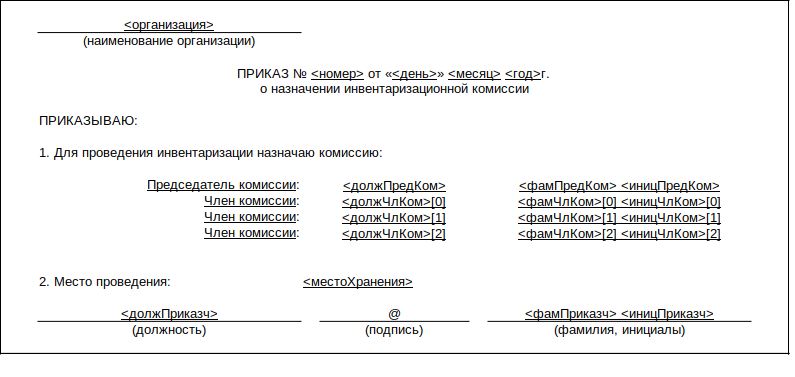
\includegraphics[width=18cm]
    {assets/ARIS/GeneralDiagram/layouts/ГП_ДОК_ПриказСозданияИнвентКомиссии.png}

    \caption{Макет оперативного документа <<Приказ о создании инвентаризационной комиссии>>}

    \label{fig:GP_DOC_Prikaz_layout}
\end{figure}

\begin{figure}[!hp]
    \centering

    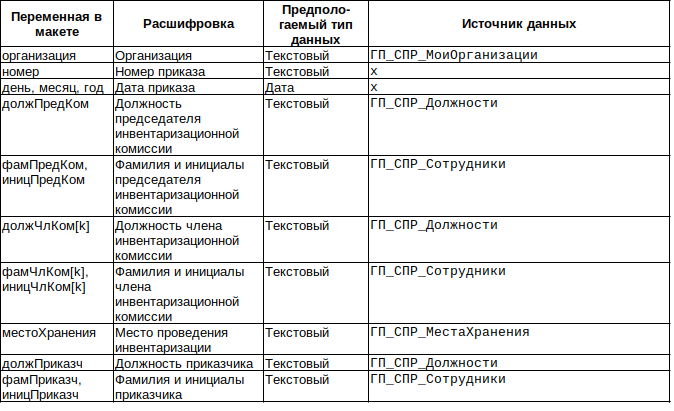
\includegraphics[width=18cm]
    {assets/ARIS/GeneralDiagram/dict/ГП_ДОК_ПриказСозданияИнвентКомиссии_словарь.png}

    \caption{Словарь данных оперативного документа <<Приказ о создании инвентаризационной комиссии>>}

    \label{fig:GP_DOC_Prikaz_data}
\end{figure}

\begin{figure}[!h]
    \centering

    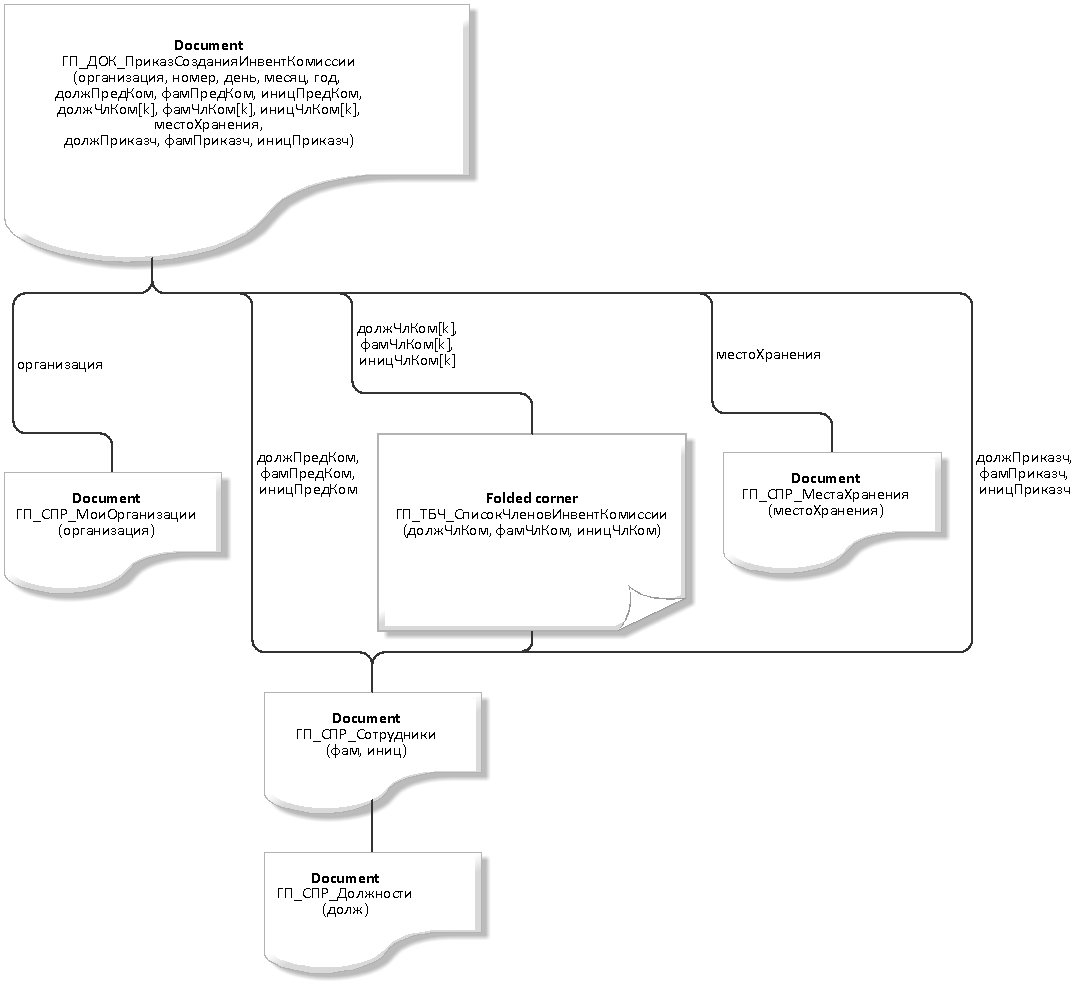
\includegraphics[width=18cm]
    {assets/ARIS/GeneralDiagram/relations/ГП_ДОК_ПриказСоздИнвентКомиссии.png}

    \caption{Схема информационной связи оперативного документа <<Приказ о создании инвентаризационной комиссии>>}

    \label{fig:GP_DOC_Prikaz_relations}
\end{figure}

\newpage

% = = = = = = = = = = = = = = = = = = = = = = = = = = = = = = = =

\subsubsection*{Оперативный документ <<Инвентаризационная опись>>}

Оперативный документ <<Инвентаризационная опись>>
- документ, в котором отображаются результаты инвентаризации. Основан на документе <<Приказ о создании инвентаризационной комиссии>>.
Документ представлен в виде
макета (см.~рисунок~\ref{fig:GP_DOC_Invent_layout}),
словаря данных (см.~рисунок~\ref{fig:GP_DOC_Invent_data})
и схемы связей (см.~рисунок~\ref{fig:GP_DOC_Invent_relations}) представленной методологией ARIS нотацией <<General Diagram>>.

\begin{figure}[!hp]
    \centering

    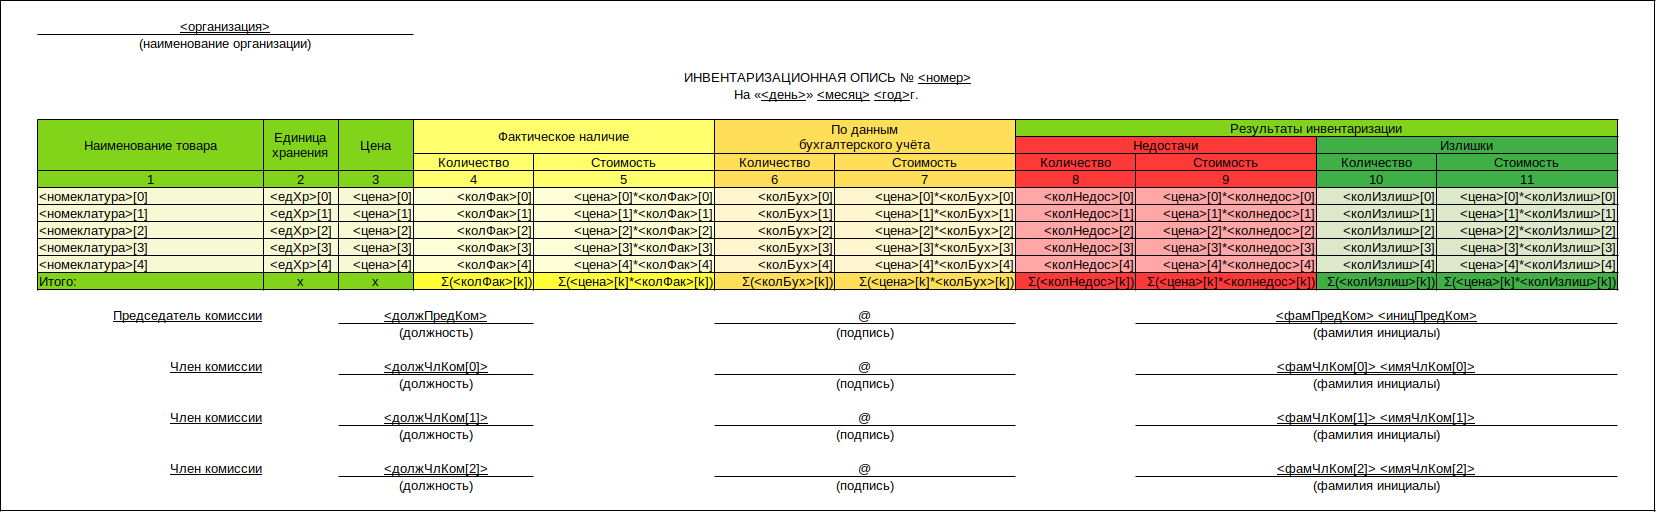
\includegraphics[width=18cm]
    {assets/ARIS/GeneralDiagram/layouts/ГП_ДОК_ИнвентОпись.png}

    \caption{Макет оперативного документа <<Инвентаризационная опись>>}

    \label{fig:GP_DOC_Invent_layout}
\end{figure}

\begin{figure}[!hp]
    \centering

    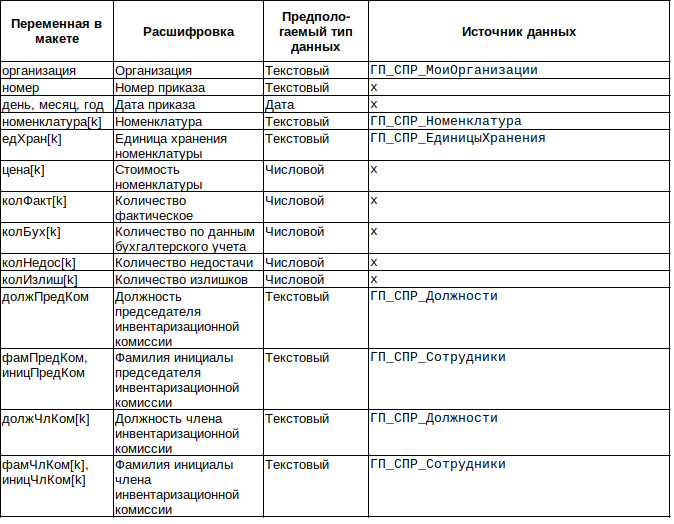
\includegraphics[width=18cm]
    {assets/ARIS/GeneralDiagram/dict/ГП_ДОК_ИнвентОпись_словарь.png}

    \caption{Словарь данных документа <<Инвентаризационная опись>>}

    \label{fig:GP_DOC_Invent_data}
\end{figure}


\begin{figure}[!h]
    \centering

    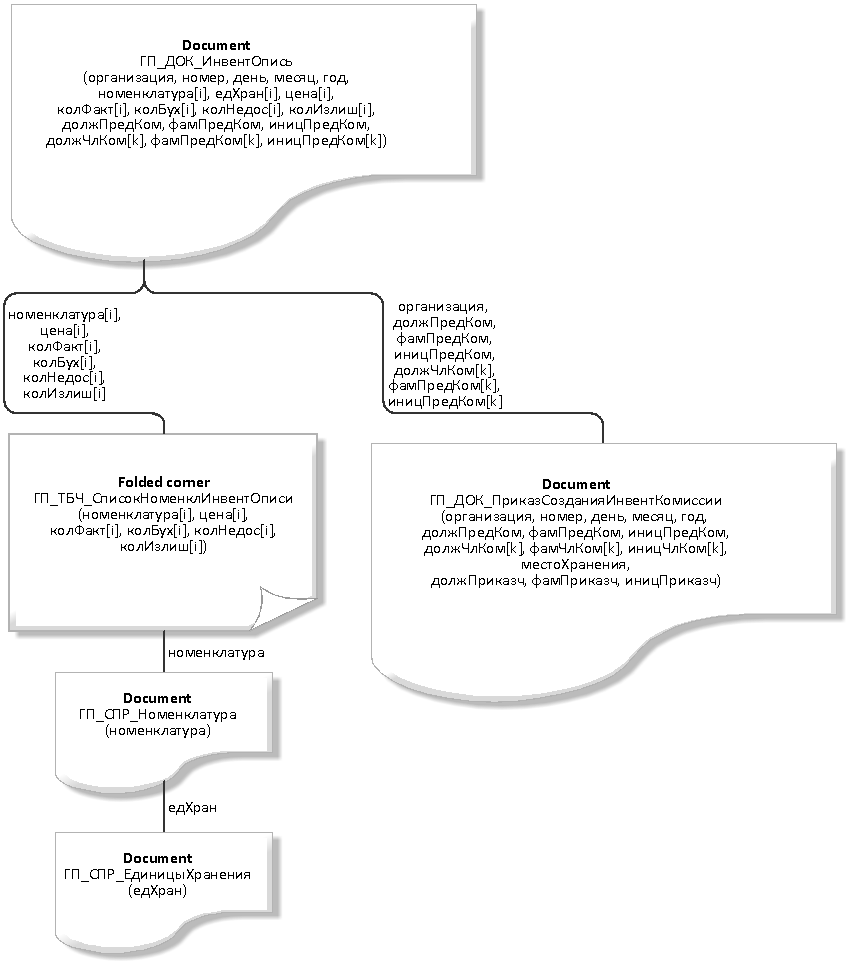
\includegraphics[height=12cm]
    {assets/ARIS/GeneralDiagram/relations/ГП_ДОК_ИнвентОпись.png}

    \caption{Схема информационной связи оперативного документа <<Инвентаризационная опись>>}

    \label{fig:GP_DOC_Invent_relations}
\end{figure}

% = = = = = = = = = = = = = = = = = = = = = = = = = = = = = = = =

\newpage

\subsubsection*{Отчёт <<Акт об инвентаризации>>}

Отчёт <<Акт об инвентаризации>>
- формируется после проведения инвентаризации. Макет изображен на рис.~\ref{fig:GP_REP_ActInvent_layout}.
Отчет представлен в виде схемы связей на рис.~\ref{fig:GP_REP_ActInvent_relations} представленной методологией ARIS нотацией <<General Diagram>>.

% Состоит отчёт из двух документов:
% \begin{itemize}
%     \item документ <<Приказ о создании инвентаризационной комиссии>>;
%     \item документ <<Инвентаризационная опись>>.
% \end{itemize}

\begin{figure}[!h]
    \centering

    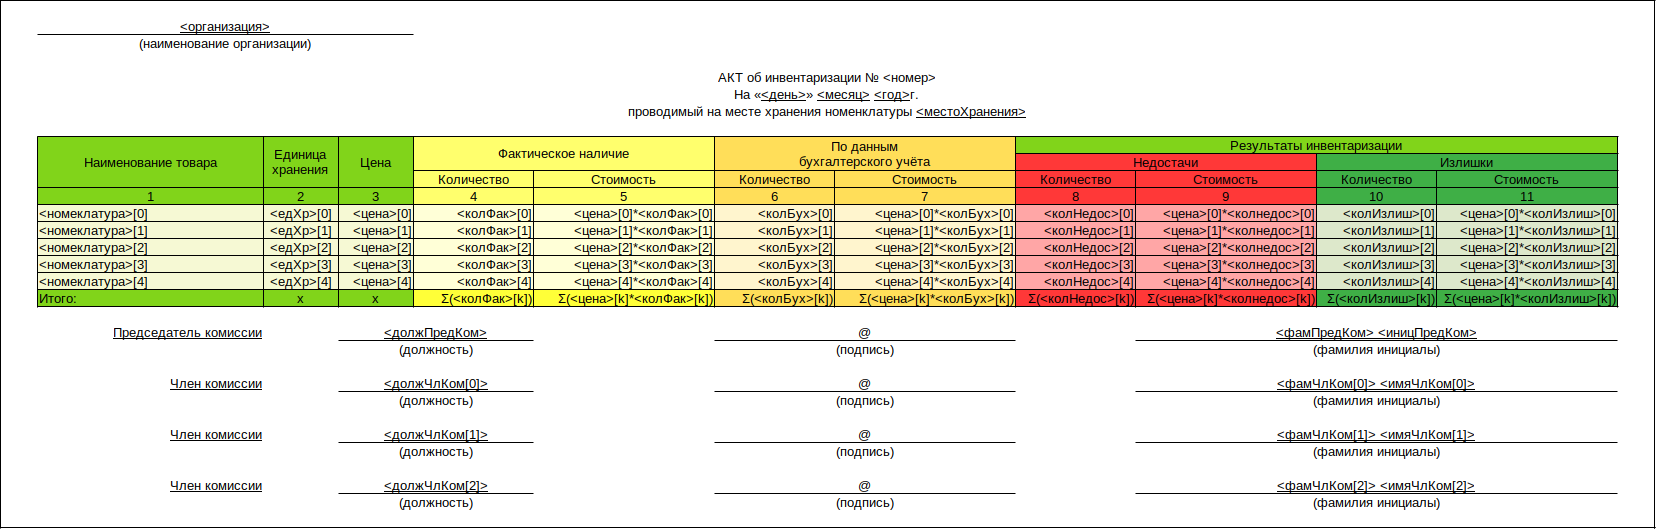
\includegraphics[width=18cm]
    {assets/ARIS/GeneralDiagram/layouts/ГП_ОТЧ_АктОбИнвентаризации.png}

    \caption{Макет отчета <<Акт об инвентаризации>>}

    \label{fig:GP_REP_ActInvent_layout}
\end{figure}

\begin{figure}[!hp]
    \centering

    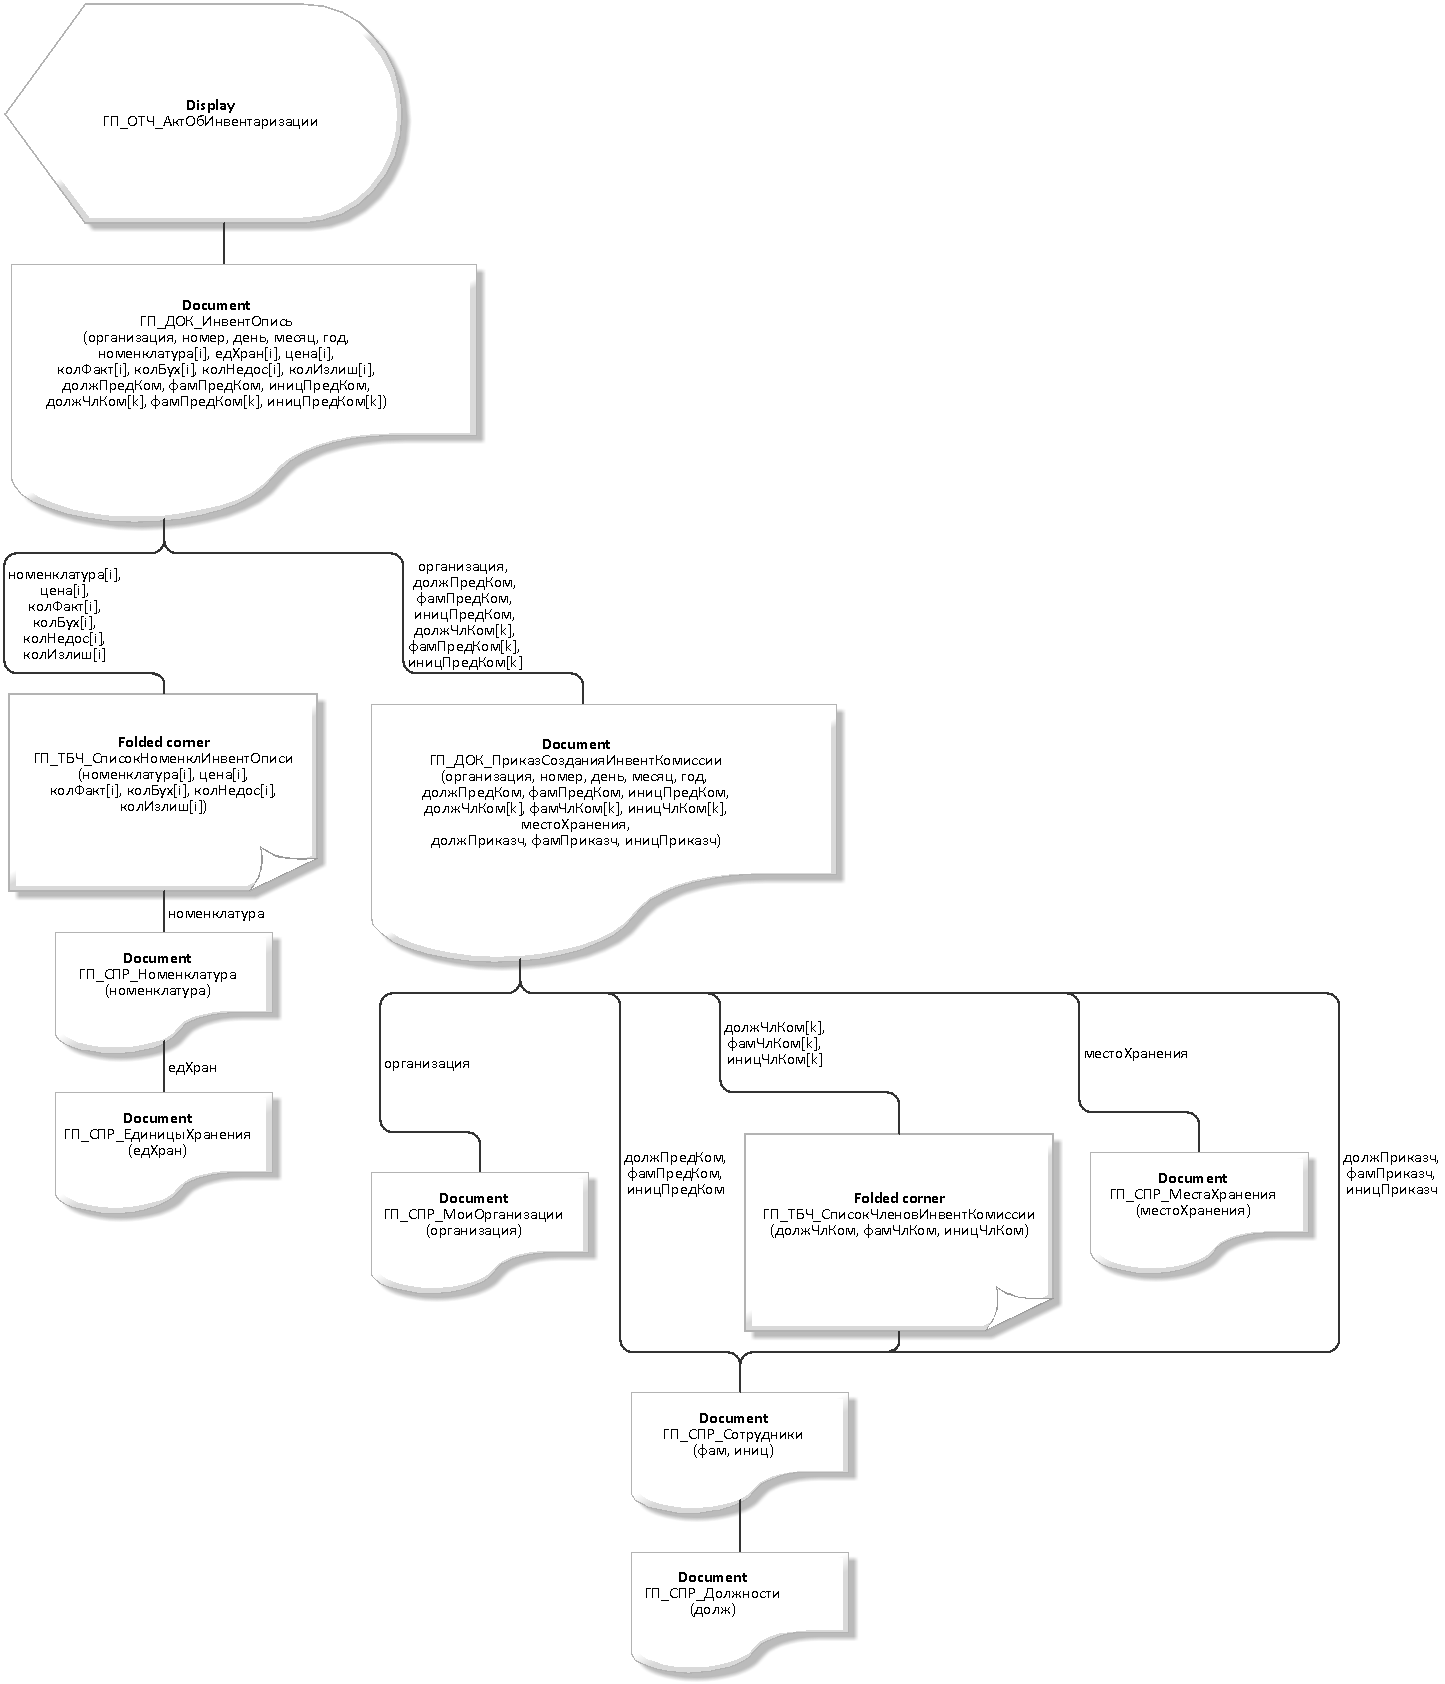
\includegraphics[width=18cm]
    {assets/ARIS/GeneralDiagram/relations/ГП_ОТЧ_АктОбИнвентаризации.png}

    \caption{Схема информационной связи оперативного документа <<Инвентаризационная опись>>}

    \label{fig:GP_REP_ActInvent_relations}
\end{figure}

% = = = = = = = = = = = = = = = = = = = = = = = = = = = = = = = =

\newpage
\subsection{Модель бизнес-процесса объекта автоматизации}

\textbf{Процесс} - любая деятельность, в которой используются ресурсы для преобразования входов в выходы.
Зачастую представляет из себя совокупность взаимосвязанных и совершенных работ,
в которых результаты одной работы являются началом другой работы,
образуя цепочку внутрненних поставщиков и потребителей.

\textbf{Бизнес-процесс} - устойчивая и целенаправленная совокупность взаимосвязанных видов деятельности,
которая по определённой технологии преобразует входной сигнал в выходной, представляющий ценность для потребителя.

\textbf{eEPC} - нотация для проектирования бизнес-процессов.
Данная нотация ARIS представляет бизнес-процесс как цепочку событий и действий (функций).
Каждое действие инициализируется и завершается событием.
Основные элементы изображены на рис.~\ref{fig:BusinessProccessElements}.

\begin{figure}[!h]
    \centering
    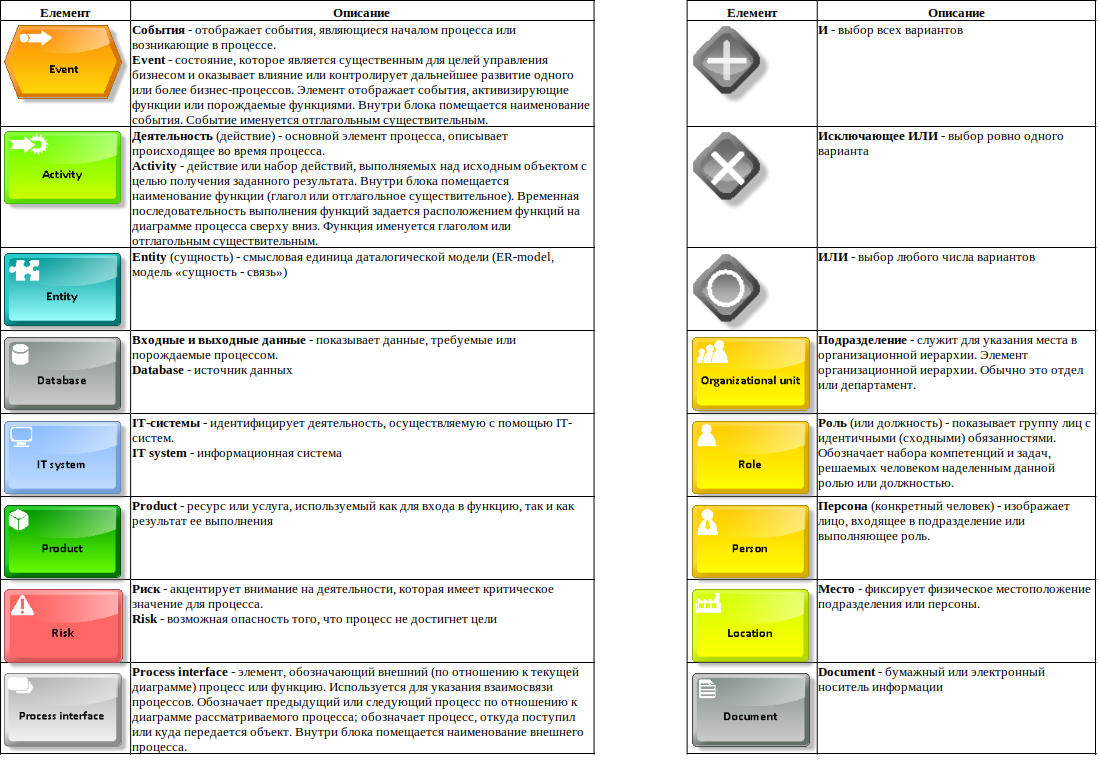
\includegraphics[width=18cm]
    {assets/ARIS/BusinessProcess/Elements/BusinessProccessElements.png}
    \caption{Основные элементы бизнес-процесса}
    \label{fig:BusinessProccessElements}
\end{figure}

\newpage

Модель бизнесс-процесса ОА <<Инвентаризация>> для ИС <<Косметический салон>> представлена методологией Business Process
с использованием нотацией ARIS (спроектированна с использованием ARIS Express 2.4 \cite{ArisExpress} нотацией <<Business Process>>) 
(см.~рисунок~\ref{fig:ARIS_BusinessProcess}).
Бизнес процесс соответствует функциональному дереву. Функции в функциональной модели совпадают с деятельностью в модели бизнес-процесса.

\begin{figure}[!h]
    \centering

    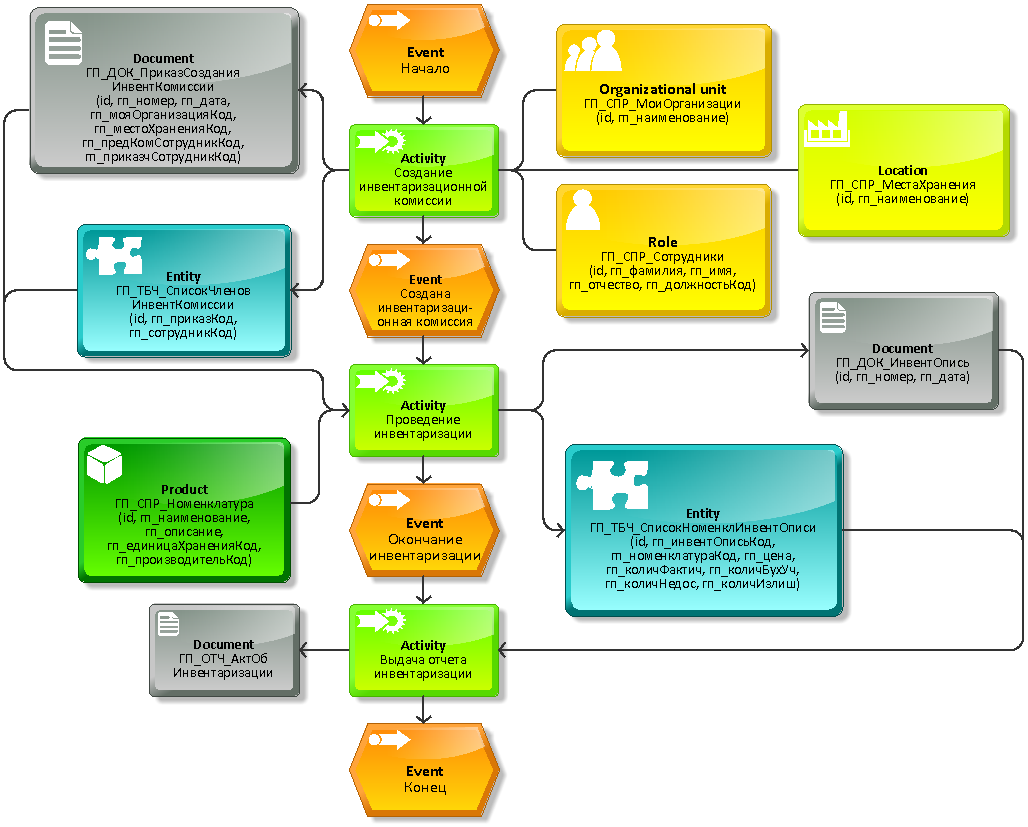
\includegraphics[width=18cm]
    {assets/ARIS/BusinessProcess/ArisBusinessProcess.png}

    \caption{Модель бизнес-процесса объекта автоматизации «Инвентаризация» для подсистемы <<Косметический салон>>}

    \label{fig:ARIS_BusinessProcess}
\end{figure}

\newpage
